\documentclass[11pt,a4paper]{article}
\usepackage[margin=1in]{geometry}
\usepackage{hyperref}
\usepackage{parskip}
\usepackage{enumitem}
\usepackage{booktabs}
\usepackage{tabularx}
\usepackage{float}
\usepackage{tikz}
\usetikzlibrary{shapes.geometric, arrows.meta, positioning, calc}

\newcommand{\shipped}{Shipped}
\newcommand{\partialstatus}{Partial}
\newcommand{\planned}{Planned}

\title{\textbf{SwarmState Technical Specification v2.0}}
\author{grave0x}
\date{2026-09-01}

\begin{document}

\maketitle
\tableofcontents
\clearpage

\section{Introduction}
SwarmState is a local-first, self-improving edge intelligence platform. It couples a deterministic C kernel with a registry-driven orchestrator, a peer-to-peer mesh, and a modular UI kit to provide constrained, private, and low-cost AI-assisted operations. The system is designed for offline and remote environments, with optional cloud escalation only when explicitly enabled.

This document is the executive and reference overview. The full consolidated design is \texttt{spec.md} (Master Technical Specification v2.0); detailed component specs live in \texttt{docs/}. Statuses below are as built on 2026-09-01.

\subsection{Core Principles}
\begin{itemize}
    \item \textbf{Mechanical containment}: The kernel enforces safety rules in C, not through prompts.
    \item \textbf{Context is contained}: The LLM sees only summaries, diffs, and plans---never the full state (~62-byte prompts on routine tasks).
    \item \textbf{Semantic feedback}: Oracles judge task success, and the registry learns from those outcomes.
    \item \textbf{Default-deny mesh}: Nodes and pools must be explicitly trusted.
    \item \textbf{Human governance}: High-risk actions require authorization and recorded reasons.
\end{itemize}

\section{Component Status}
\begin{center}
\begin{tabularx}{\textwidth}{l l X}
\toprule
\textbf{Component} & \textbf{Status} & \textbf{Notes} \\
\midrule
C Kernel & \shipped & Ops, governance gate, path safety; 175 C checks \\
Registry & \shipped & Semantic, temporal, per-pool partitions \\
Orchestrator & \shipped & Route$\rightarrow$see$\rightarrow$diagnose$\rightarrow$rescue$\rightarrow$learn loop \\
Mesh & \shipped & TCP + Tailcat + LoRa (sim); pools, bridges, multi-homing \\
Governance & \shipped & Auth tokens, recorded reasons, multi-party, audit ledger \\
Windows Node & \shipped & Self-contained zip (node exe + kernel DLL + web UI) \\
UI Kit & \partialstatus & v1 shell + 6 core widgets; full catalogue planned \\
Identity / Roles & \partialstatus & Signed identity store (DORMANT); role gating on roadmap \\
Embedded Inference & \planned & llama.cpp integration (spec v1) \\
Support / Ops Layer & \planned & MSP dashboard, Watch mode \\
Native App & \planned & Standalone-first app \\
Radio Backbone & \planned & Licensed point-to-point / LMR \\
\bottomrule
\end{tabularx}
\end{center}

\section{System Architecture}
The system is composed of six logical layers:

\begin{center}
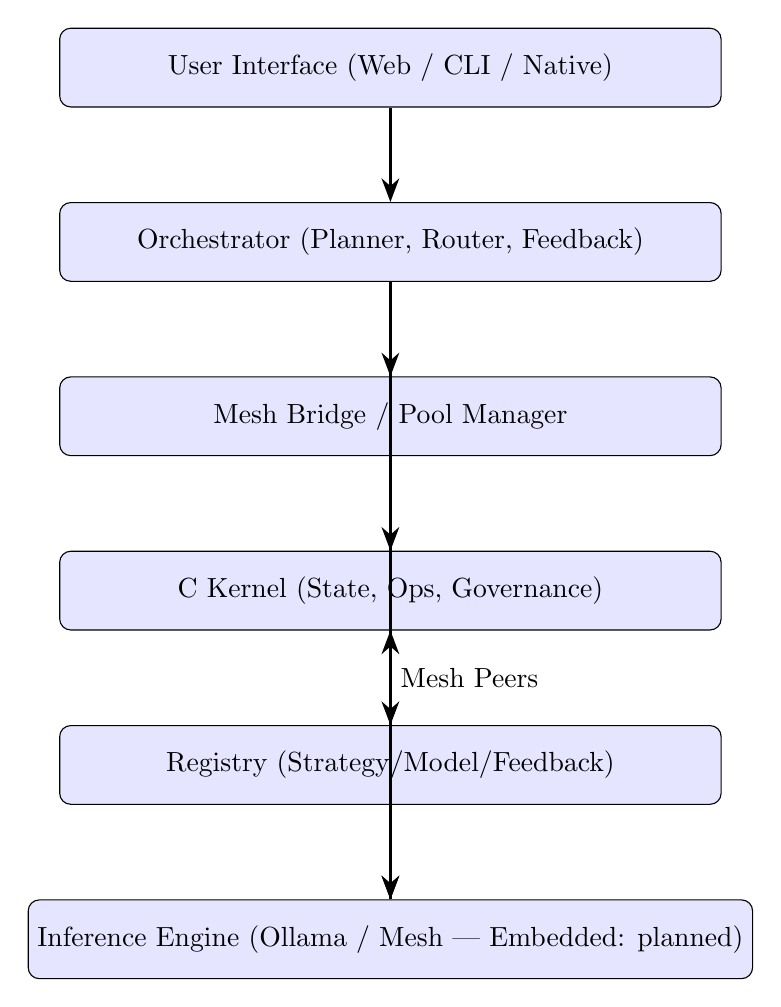
\begin{tikzpicture}[
    node distance=1.2cm,
    layer/.style={draw, rounded corners, minimum width=8.4cm, minimum height=1cm, align=center, fill=blue!10},
    arrow/.style={-{Stealth[length=3mm]}, thick}
]
\node[layer] (ui) {User Interface (Web / CLI / Native)};
\node[layer, below=of ui] (orch) {Orchestrator (Planner, Router, Feedback)};
\node[layer, below=of orch] (bridge) {Mesh Bridge / Pool Manager};
\node[layer, below=of bridge] (kernel) {C Kernel (State, Ops, Governance)};
\node[layer, below=of kernel] (registry) {Registry (Strategy/Model/Feedback)};
\node[layer, below=of registry] (infer) {Inference Engine (Ollama / Mesh --- Embedded: planned)};

\draw[arrow] (ui) -- (orch);
\draw[arrow] (orch) -- (bridge);
\draw[arrow] (bridge) -- (kernel);
\draw[arrow] (kernel) -- (registry);
\draw[arrow] (orch) -- (infer);
\draw[arrow] (infer) -- (kernel);
\draw[arrow, dashed] (bridge) -- node[right] {Mesh Peers} (infer);
\end{tikzpicture}
\end{center}

\subsection{Kernel}
The kernel is a C library and daemon that owns the local state and executes plans. It exposes a small, typed set of operations and enforces:
\begin{itemize}
    \item Path containment via \texttt{realpath} and \texttt{O\_NOFOLLOW}
    \item Binary allowlists and argument validation for \texttt{EXECUTE}
    \item Schema validation for all incoming plans
    \item Governance checks for high-risk ops (token + reason)
\end{itemize}

\subsection{Kernel Operations}
\begin{center}
\begin{tabularx}{\textwidth}{l l X}
\toprule
\textbf{Op} & \textbf{Risk} & \textbf{Purpose} \\
\midrule
\texttt{SS\_OP\_READ} & Low & Read file contents (optional line range) \\
\texttt{SS\_OP\_WRITE} & Medium & Write file contents (blind-write guard applies) \\
\texttt{SS\_OP\_GREP} & Low & POSIX ERE search over a path \\
\texttt{SS\_OP\_DIFF} & Low & Git diff (repo or one path) \\
\texttt{SS\_OP\_STATUS} & Low & Git status --porcelain \\
\texttt{SS\_OP\_EXECUTE} & High & Whitelisted binary, filtered args (allowlist) \\
\texttt{SS\_OP\_AST\_PARSE} / \texttt{SS\_OP\_AST\_QUERY} & Low & Tree-sitter parse / query \\
\texttt{SS\_OP\_SYMBOL\_SUMMARY} & Low & Doc-layer symbol summaries (SYMBOLIC strategy) \\
\texttt{FILE\_REQUEST} / \texttt{MESH\_SEND} & Medium & Mesh/bridge layer: serve file, relay op (bridge policy) \\
\bottomrule
\end{tabularx}
\end{center}

\section{Registry and Learning}
\subsection{Key Structure}
A persistent key-value store that tracks success rates per task signature, strategy, model, and resource context. Keys follow a deterministic pattern:

\begin{center}
\begin{tabularx}{\textwidth}{l X}
\toprule
\textbf{Key} & \textbf{Meaning} \\
\midrule
\texttt{STRAT:<plan-sig>:<strategy>} & Strategy success rate \\
\texttt{STRAT:<plan-sig>:<strategy>:<model>} & Per-model strategy success \\
\texttt{MODEL:q:<query-sig>:<model>} & Query-level model routing \\
\texttt{POOL:<pool-id>:STRAT:<sig>:<strategy>} & Cross-pool learning partition (source-tagged) \\
\texttt{<key>} value & \texttt{(fb\_ok, fb\_count)} plus timing stats \\
temporal tags & \texttt{min / max / last\_ts} freshness window \\
\bottomrule
\end{tabularx}
\end{center}

\subsection{Learning Loop}
\begin{enumerate}
    \item User query $\rightarrow$ task signature computed.
    \item Router checks the registry for a proven strategy/model.
    \item Plan generated and executed.
    \item Oracle scores the semantic outcome.
    \item Feedback written to the registry (local and bridged).
\end{enumerate}

\subsection{Cross-Node Propagation and Integrity}
Mesh ops carry registry updates. Bridged learning is source-tagged (\texttt{POOL:<src>:...}) and never pollutes the local partition. \textbf{Planned:} a hash-chain journal with node-signed entries makes poisoning detectable (see \S\ref{sec:security}).

\section{Orchestrator and Plan Generation}
\subsection{Flow}
\begin{center}
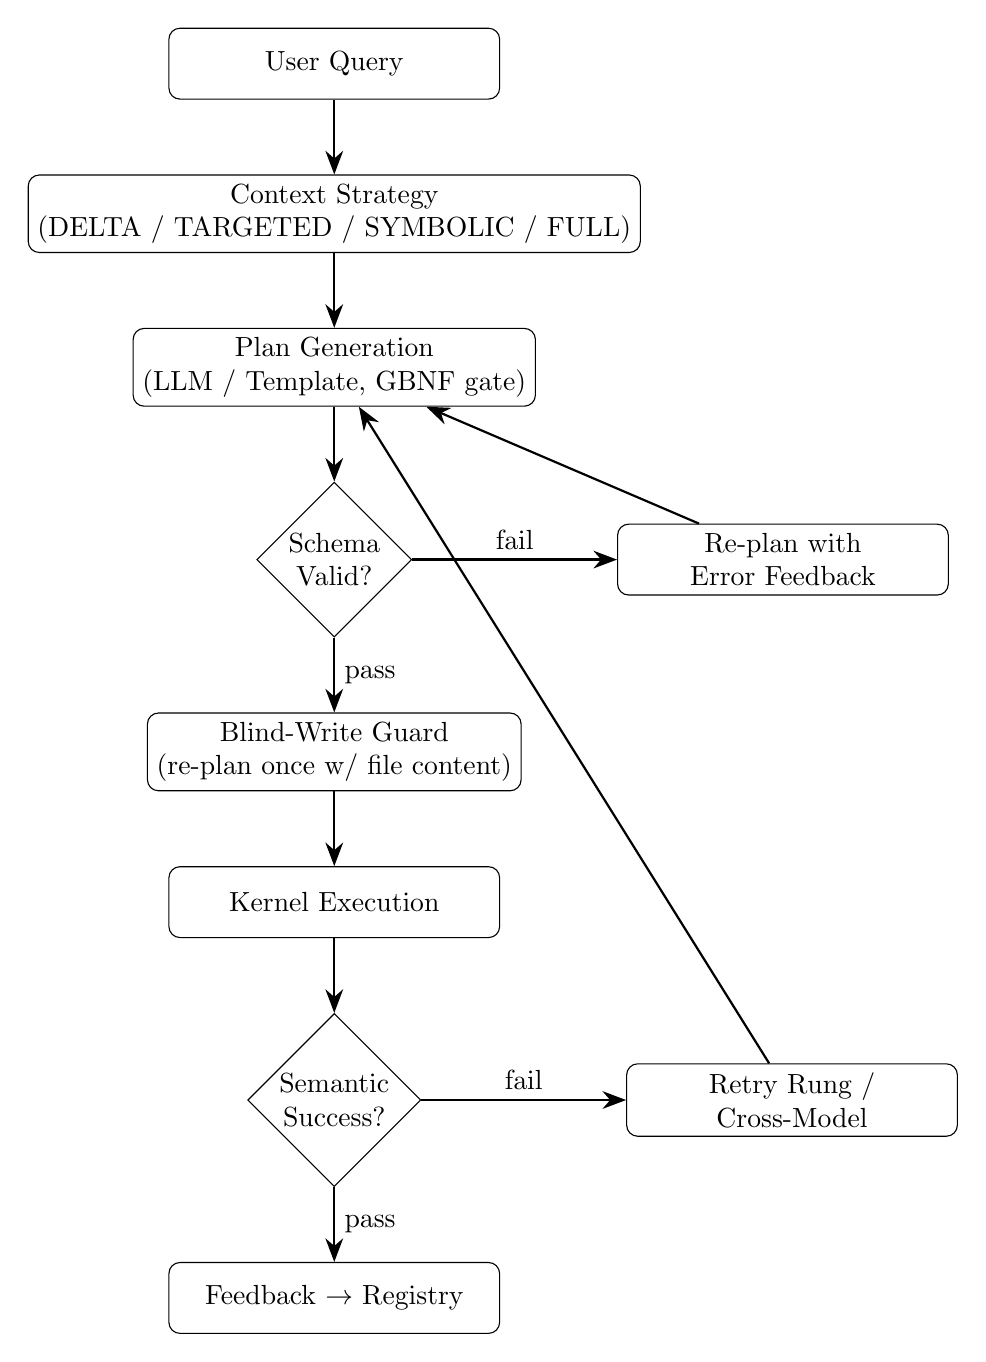
\begin{tikzpicture}[
    node distance=0.95cm,
    box/.style={draw, rounded corners, minimum width=4.2cm, minimum height=0.9cm, align=center},
    decision/.style={diamond, draw, minimum width=1.6cm, minimum height=0.9cm, align=center, inner sep=1pt},
    arrow/.style={-{Stealth[length=3mm]}, thick}
]
\node[box] (start) {User Query};
\node[box, below=of start] (strat) {Context Strategy\\ (DELTA / TARGETED / SYMBOLIC / FULL)};
\node[box, below=of strat] (plan) {Plan Generation\\ (LLM / Template, GBNF gate)};
\node[decision, below=of plan] (valid) {Schema\\ Valid?};
\node[box, right=2.6cm of valid] (replan) {Re-plan with\\ Error Feedback};
\node[box, below=of valid] (write) {Blind-Write Guard\\ (re-plan once w/ file content)};
\node[box, below=of write] (exec) {Kernel Execution};
\node[decision, below=of exec] (ok) {Semantic\\ Success?};
\node[box, right=2.6cm of ok] (retry) {Retry Rung /\\ Cross-Model};
\node[box, below=of ok] (learn) {Feedback $\rightarrow$ Registry};

\draw[arrow] (start) -- (strat);
\draw[arrow] (strat) -- (plan);
\draw[arrow] (plan) -- (valid);
\draw[arrow] (valid) -- node[above] {fail} (replan);
\draw[arrow] (replan) -- (plan);
\draw[arrow] (valid) -- node[right] {pass} (write);
\draw[arrow] (write) -- (exec);
\draw[arrow] (exec) -- (ok);
\draw[arrow] (ok) -- node[above] {fail} (retry);
\draw[arrow] (retry) -- (plan);
\draw[arrow] (ok) -- node[right] {pass} (learn);
\end{tikzpicture}
\end{center}

\subsection{Retry and Rescue}
\begin{itemize}
    \item Schema failure $\rightarrow$ re-plan with validation errors fed back.
    \item Execution failure $\rightarrow$ re-plan with the kernel error.
    \item Both fail $\rightarrow$ cross-model retry (a different brain).
    \item Still failing $\rightarrow$ escalate to cloud or a human.
\end{itemize}

\subsection{The Central Loop}
\begin{center}
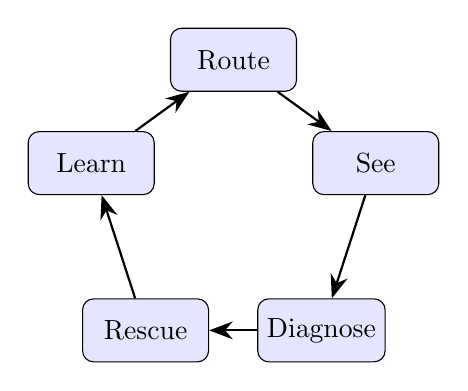
\begin{tikzpicture}[
    loopnode/.style={draw, rounded corners, minimum width=1.6cm, minimum height=0.8cm, align=center, fill=blue!10},
    arrow/.style={-{Stealth[length=3mm]}, thick}
]
\node[loopnode] (route) at (90:1.9) {Route};
\node[loopnode] (see) at (18:1.9) {See};
\node[loopnode] (diag) at (-54:1.9) {Diagnose};
\node[loopnode] (rescue) at (-126:1.9) {Rescue};
\node[loopnode] (learn) at (162:1.9) {Learn};

\draw[arrow] (route) -- (see);
\draw[arrow] (see) -- (diag);
\draw[arrow] (diag) -- (rescue);
\draw[arrow] (rescue) -- (learn);
\draw[arrow] (learn) -- (route);
\end{tikzpicture}
\end{center}

\section{Mesh and Federation}
\subsection{Transports}
\begin{center}
\begin{tabularx}{\textwidth}{l l X}
\toprule
\textbf{Transport} & \textbf{Status} & \textbf{Use Case} \\
\midrule
TCP & \shipped & LAN \\
Tailcat & \shipped & Encrypted WAN without control plane (WireGuard + DERP) \\
LoRa & Partial (sim) & Long-range, low-bandwidth; real hardware on roadmap \\
Point-to-point radio & \planned & Licensed backbone / LMR \\
\bottomrule
\end{tabularx}
\end{center}

\subsection{Mesh Message Types}
Implemented on the node daemon (\texttt{meshd.py}): \texttt{hello}, \texttt{join}, \texttt{join\_ok}, \texttt{join\_denied}, \texttt{member\_added}, \texttt{capability}, \texttt{req}, \texttt{resp}, \texttt{file\_request}, \texttt{file\_response}, \texttt{lora\_share}, \texttt{op}. Spec'd for the full vision: \texttt{heartbeat}, \texttt{capability\_announce}, \texttt{inference\_request}, \texttt{inference\_response}, \texttt{state\_diff}.

\subsection{Pools and Bridges}
\begin{itemize}
    \item \textbf{Pool}: a set of nodes sharing a trust boundary.
    \item \textbf{Bridge}: a scoped connection between two pools. Policy scopes allowed message types (default: registry learning only), task-signature globs, TTL, and data minimization (MODEL routing keys stay local). Both sides must accept.
    \item \textbf{Multi-homing}: a node may belong to several pools, each with its own registry partition and identity.
\end{itemize}

\begin{center}
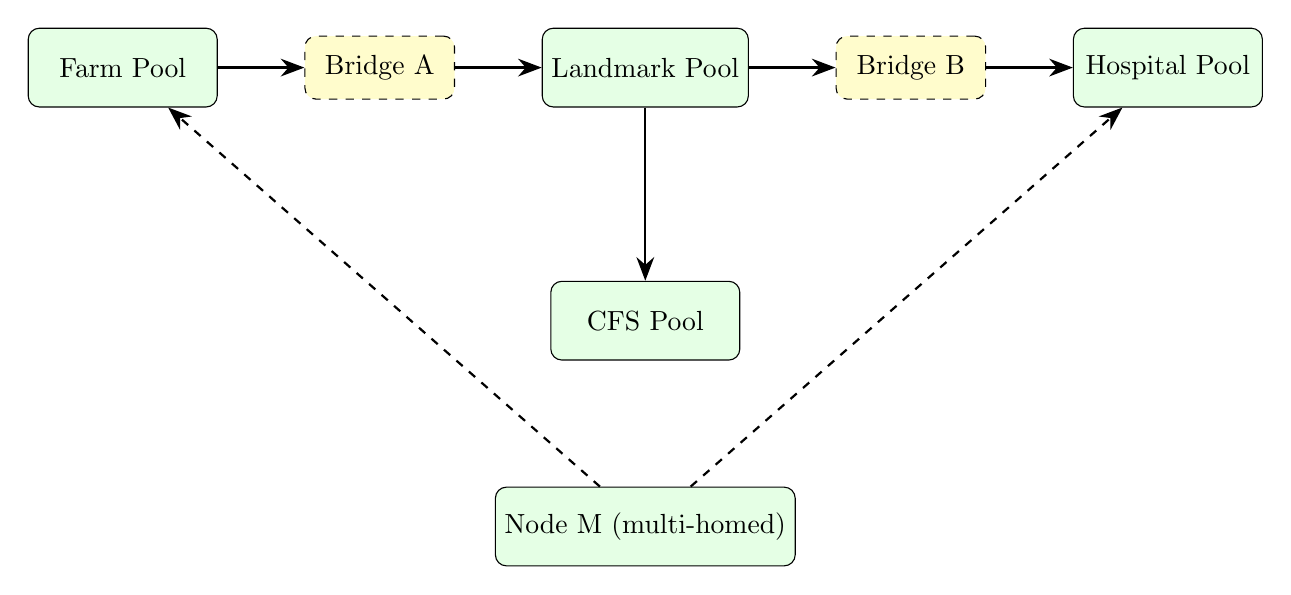
\begin{tikzpicture}[
    node distance=1.4cm,
    pool/.style={draw, rounded corners, minimum width=2.4cm, minimum height=1cm, align=center, fill=green!10},
    bridge/.style={draw, dashed, rounded corners, minimum width=1.9cm, minimum height=0.8cm, align=center, fill=yellow!20},
    arrow/.style={-{Stealth[length=3mm]}, thick}
]
\node[pool] (farm) {Farm Pool};
\node[bridge, right=1.1cm of farm] (b1) {Bridge A};
\node[pool, right=1.1cm of b1] (landmark) {Landmark Pool};
\node[bridge, right=1.1cm of landmark] (b2) {Bridge B};
\node[pool, right=1.1cm of b2] (hospital) {Hospital Pool};
\node[pool, below=2.2cm of landmark] (cfs) {CFS Pool};
\node[pool, below=1.6cm of cfs] (multi) {Node M (multi-homed)};

\draw[arrow] (farm) -- (b1);
\draw[arrow] (b1) -- (landmark);
\draw[arrow] (landmark) -- (b2);
\draw[arrow] (b2) -- (hospital);
\draw[arrow] (landmark) -- (cfs);
\draw[arrow, dashed] (multi) -- (farm);
\draw[arrow, dashed] (multi) -- (hospital);
\end{tikzpicture}
\end{center}
\smallskip

\subsection{Inference Broker}
Provider nodes broadcast capability announcements (model, load, freshness). Consumers send inference requests; the broker scores candidates and routes to the best provider, with fallback to local inference when no provider is available.

\section{Governance and Safety}
\subsection{Principles}
\begin{itemize}
    \item The model never acts directly.
    \item High-risk ops require authorization.
    \item All decisions are audited.
\end{itemize}

Risk tiers: SAFE (read-only), WRITE, EXEC, ACTUATE (reserved for future \texttt{CONTROL\_*} ops). Governed ops need a valid HMAC-SHA256 token (\texttt{ss:<role>:<expiry>}, short TTL, constant-time verify) \emph{and} a recorded reason. The reason is checked first, so the denial tells the user what to fix.

\subsection{Authorization Flow}
\begin{center}
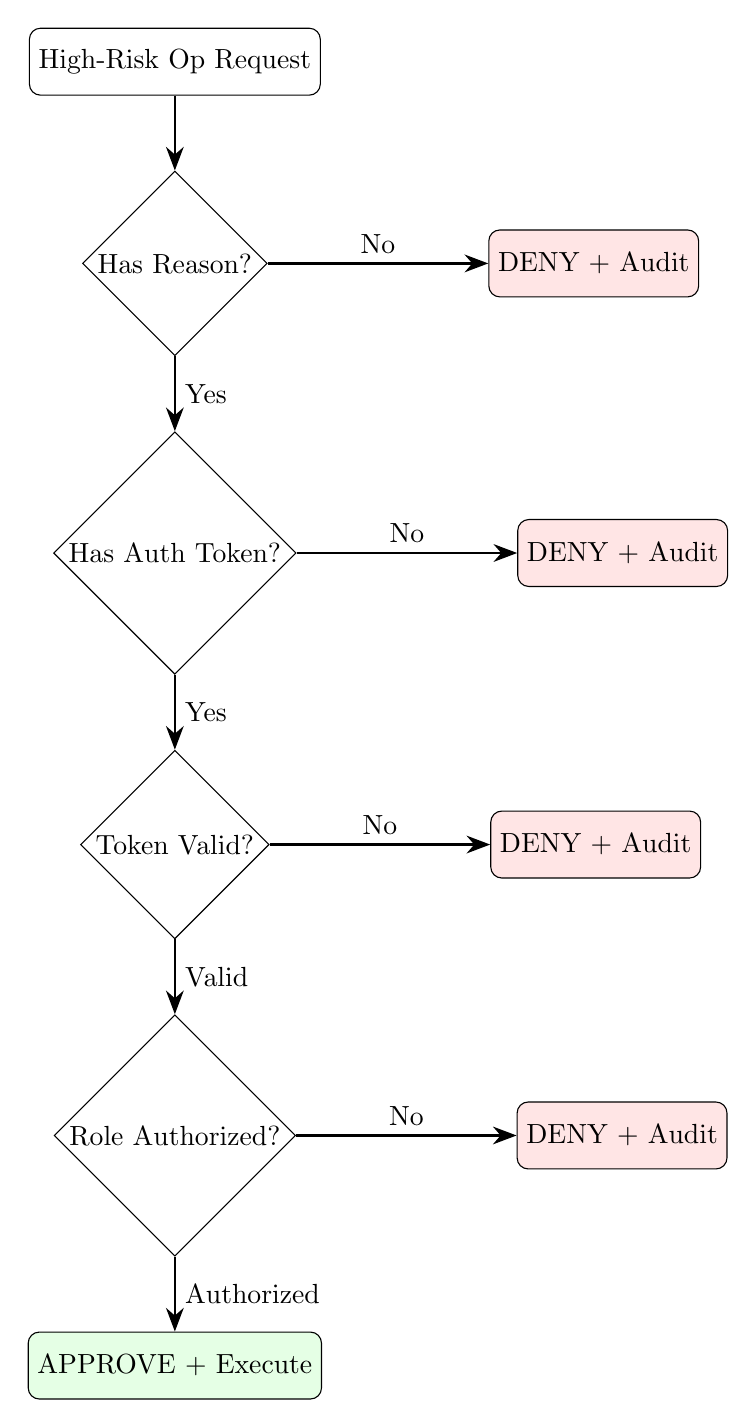
\begin{tikzpicture}[
    node distance=0.95cm,
    box/.style={draw, rounded corners, minimum width=3.4cm, minimum height=0.85cm, align=center},
    decision/.style={diamond, draw, minimum width=1.5cm, minimum height=0.85cm, align=center, inner sep=1pt},
    deny/.style={draw, rounded corners, fill=red!10, minimum width=2.6cm, minimum height=0.85cm, align=center},
    arrow/.style={-{Stealth[length=3mm]}, thick}
]
\node[box] (req) {High-Risk Op Request};
\node[decision, below=of req] (reason) {Has Reason?};
\node[deny, right=2.8cm of reason] (d1) {DENY + Audit};
\node[decision, below=of reason] (auth) {Has Auth Token?};
\node[deny, right=2.8cm of auth] (d2) {DENY + Audit};
\node[decision, below=of auth] (valid) {Token Valid?};
\node[deny, right=2.8cm of valid] (d3) {DENY + Audit};
\node[decision, below=of valid] (role) {Role Authorized?};
\node[deny, right=2.8cm of role] (d4) {DENY + Audit};
\node[box, below=of role, fill=green!10] (approve) {APPROVE + Execute};

\draw[arrow] (req) -- (reason);
\draw[arrow] (reason) -- node[above] {No} (d1);
\draw[arrow] (reason) -- node[right] {Yes} (auth);
\draw[arrow] (auth) -- node[above] {No} (d2);
\draw[arrow] (auth) -- node[right] {Yes} (valid);
\draw[arrow] (valid) -- node[above] {No} (d3);
\draw[arrow] (valid) -- node[right] {Valid} (role);
\draw[arrow] (role) -- node[above] {No} (d4);
\draw[arrow] (role) -- node[right] {Authorized} (approve);
\end{tikzpicture}
\end{center}

\subsection{Multi-Party Approval and Audit}
For cross-pool actions, every required authority must present a valid token; the gate checks all roles and always audits. Every approval/denial is appended to the ledger with timestamp, user, role, op, and reason. The ledger is append-only; hash-chain tamper evidence is planned (see \S\ref{sec:security}).

\section{Support and Operations}
\label{sec:support}
Role-based access control enables MSP-style management of remote nodes:

\begin{center}
\begin{tabularx}{\textwidth}{l l X}
\toprule
\textbf{Role} & \textbf{Scope} & \textbf{Typical Actions} \\
\midrule
Field & Single device & Use assistant, view tasks, request help \\
Support (MSP) & Managed client pool & Diagnostics, rejoin, invite, escalate \\
Architect & Full system & Updates, rollback, audit, cross-pool \\
Watch & Automatic & Health checks, safe self-remediation \\
\bottomrule
\end{tabularx}
\end{center}

\textbf{Watch mode}: each node monitors its own health (disk, memory, CPU, registry, mesh). Deviations trigger alerts; a finite set of safe auto-fixes may run (restart link, rejoin pool, resend ops)---all logged and reversible. \textbf{Prompt-based administration} translates natural-language technician commands into structured, kernel-validated ops. Status: roles and flows are specified; enforcement (role gating, Watch) is on the roadmap.

\section{User Interface}
\label{sec:ui}
The UI is a web app served from the local node: a widget shell plus role-based widgets.

\subsection{Widget Catalogue}
Map, Task List, Alert Banner, Team Roster, Vitals/Sensor Panel, Governance Console, Voice Input, Knowledge Search, QR/Invite, Status Dashboard.

\subsection{Role Views}
\begin{center}
\begin{tabularx}{\textwidth}{l X}
\toprule
\textbf{Role} & \textbf{Typical Widgets} \\
\midrule
Field Worker & Map, Task List, Alert Banner, Voice Input \\
Supervisor & Roster, Task List, Governance Console, Alerts \\
Admin & QR/Invite, Status Dashboard, Knowledge Search \\
Observer & Map, Alerts, Knowledge Search (read-only) \\
\bottomrule
\end{tabularx}
\end{center}

Layout is config-driven (\texttt{config/widgets.json}): a non-technical user sees a role-appropriate dashboard, and the layout changes by editing config, not code. Governance is enforced at the node regardless of UI role.

\section{Security Posture}
\label{sec:security}
A 67-case attack battery (kernel exec/write containment, governance, multi-party, pool/join, mesh) finished 61 PASS / 5 WEAK / 0 FAIL, with single-use invites (replay protection), reason-before-auth error paths, backslash path handling, and a registry freshness window applied. Findings: \texttt{docs/redteam-findings.md}.

\begin{center}
\begin{tabularx}{\textwidth}{l X}
\toprule
\textbf{Remaining Gap} & \textbf{Mitigation Plan} \\
\midrule
Registry tampering & Hash-chain journal with node signatures \\
LoRa encryption & AES-256-GCM with pre-shared or exchanged keys \\
Pool secret storage & OS keychain / DPAPI \\
Windows \texttt{EXECUTE} & PowerShell allowlist or service manager \\
External pen test & Schedule before production pilot \\
\bottomrule
\end{tabularx}
\end{center}

\section{Acceptance Criteria}
\begin{center}
\begin{tabularx}{\textwidth}{l l X}
\toprule
\textbf{Capability} & \textbf{Result} & \textbf{Notes} \\
\midrule
C test suite & 175 checks & \texttt{make test}; full suite adds harness/py/rg \\
Red-team battery & 67 cases & 61 PASS / 5 WEAK / 0 FAIL, PITCH\_READY \\
3-node live acceptance & PASS & Real Ollama + strict grammar gate \\
Contained prompts & $\sim$62 B & vs.\ naive 100+ KB prompts \\
Grep 10k files & $<15$ ms & auto 0.81 ms, 18x headroom \\
Batch latency & 133 $\mu$s / 5 ops & 26.7 $\mu$s per op; MVP bar $<1$ ms \\
Mesh convergence & 2 nodes $\rightarrow$ 1 hash & 2 STRAT each way, tail 4, $\sim$1.2 MB RSS \\
\bottomrule
\end{tabularx}
\end{center}

\section{Roadmap and Milestones}
\begin{itemize}
    \item \textbf{Short term (2--4 weeks):} embedded inference engine (CPU-only first); pitch demo on a clean machine; Windows \texttt{EXECUTE} implementation.
    \item \textbf{Medium term (1--3 months):} first pilot (CFS or MSP); external security review; native app alpha; registry hash-chain integrity.
    \item \textbf{Long term (3--12 months):} radio backbone trial; multi-party governance in C; full support/ops layer; community contributions.
\end{itemize}

\section{Conclusion}
SwarmState is a complete, local-first edge intelligence platform that combines mechanical safety, semantic feedback, and peer-to-peer mesh learning. It is ready for real-world pilots in agriculture, emergency services, healthcare, and remote operations. The full consolidated reference is \texttt{spec.md} (v2.0); this document tracks the same architecture and statuses.

\end{document}
